%%%%%%%%%%%%%%%%%%%%%%%%%%%%%%%%%%%%%%%%%%%%%%%%%%%%%%%%%%%%%%%%%%%%%%%%%%%%%%%

\documentclass[12pt,twocolumn,tighten]{aastex62}
%\documentclass[12pt,twocolumn,tighten,trackchanges]{aastex62}
\usepackage{amsmath,amstext,amssymb}
\usepackage[T1]{fontenc}
\usepackage{apjfonts}
\usepackage[figure,figure*]{hypcap}
\usepackage{graphics,graphicx}
\usepackage{hyperref}
\usepackage{natbib}
\usepackage[caption=false]{subfig} % for subfloat
\usepackage{enumitem} % for specific spacing of enumerate
\usepackage{epigraph}

\renewcommand*{\sectionautorefname}{Section} %for \autoref
\renewcommand*{\subsectionautorefname}{Section} %for \autoref

\newcommand{\tn}{TOI~837} % target star name
\newcommand{\pn}{TOI~837.01} % planet name
\newcommand{\cn}{IC~2602} % cluster name


%% Reintroduced the \received and \accepted commands from AASTeX v5.2.
%% Add "Submitted to " argument.
\received{\today}
\revised{---}
\accepted{---}
\submitjournal{AAS journals.}
\shorttitle{TOI~837 in IC~2602}

\begin{document}

\defcitealias{bouma_wasp4b_2019}{B19}

\title{
  Cluster Difference Imaging Photometric Survey (CDIPS) II:
  Validatation of a Jupiter-Sized Planet in IC~2602
}

\correspondingauthor{L.\,G.\,Bouma}
\email{luke@astro.princeton.edu}

%
% key authors:
%

\author[0000-0002-0514-5538]{L. G. Bouma}
\affiliation{Department of Astrophysical Sciences, Princeton
University, 4 Ivy Lane, Princeton, NJ 08540, USA}

%PENDING
\author[0000-0002-9158-7315]{R. Brahm}
\affiliation{Center of Astro-Engineering UC, Pontificia Universidad
Cat\'olica de Chile, Av. Vicu\~na Mackenna 4860, 782-0436 Macul,
Santiago, Chile}
\affiliation{Instituto de Astrof\'isica, Facultad de F\'isica,
Pontificia Universidad Cat\'olica de Chile, Av. Vicu\~na Mackenna
4860, 782-0436 Macul, Santiago, Chile}
\affiliation{Millennium Institute of Astrophysics, Av. Vicu\~na
Mackenna 4860, 782-0436 Macul, Santiago, Chile}

\author[0000-0001-8732-6166]{J. D. Hartman}
\affiliation{Department of Astrophysical Sciences, Princeton
University, 4 Ivy Lane, Princeton, NJ 08540, USA}

%PENDING
\author{J. de Leon}
\affiliation{Department of Astronomy, University of Tokyo, 7-3-1
Hongo, Bunkyo-ky, Tokyo 113-0033, Japan}

%
% SG1 contributors: ask Karen -- are there others?
%
%PENDING
\author{P. Evans}
\affiliation{El Sauce Observatory, Coquimbo Province, Chile}

%PENDING
\author[0000-0001-6588-9574]{K. A. Collins} % karenacollins@outlook.com
\affiliation{Center for Astrophysics \textbar \ Harvard \&
Smithsonian, 60 Garden St, Cambridge, MA 02138, USA}

%
% SG2 contributors
%
%PENDING
\author[0000-0002-4891-3517]{G. Zhou}
\affiliation{Center for Astrophysics \textbar \ Harvard \&
Smithsonian, 60 Garden St, Cambridge, MA 02138, USA}

%PENDING
\author[0000-0002-8964-8377]{S. N. Quinn} % squinn@cfa.harvard.edu
\affiliation{Center for Astrophysics \textbar \ Harvard \&
Smithsonian, 60 Garden St, Cambridge, MA 02138, USA}

%
% SG4 contributors
%
\author[0000-0002-0619-7639]{C.~Ziegler}
\affiliation{Dunlap Institute for Astronomy and Astrophysics,
University of Toronto, 50 St. George Street, Toronto, Ontario M5S 3H4,
Canada}

%
% UToyko team
%
%PENDING
\author[0000-0002-4881-3620]{J. Livingston}
\affiliation{Department of Astronomy, University of Tokyo, 7-3-1
Hongo, Bunkyo-ky, Tokyo 113-0033, Japan}

%
% MPIA team
%
%PENDING
\author{T. Henning}
\affiliation{Max-Planck-Institut f\"ur Astronomie, K\"onigstuhl 17,
69117 Heidelberg, Germany}

%PENDING
\author[0000-0002-5389-3944]{A. Jord\'an}
\affiliation{Facultad de Ingenier\'ia y Ciencias, Universidad Adolfo
Ib\'a\~nez, Av.\ Diagonal las Torres 2640, Pe\~nalol\'en, Santiago,
Chile}
\affiliation{Millennium Institute of Astrophysics, Av. Vicu\~na
Mackenna 4860, 782-0436 Macul, Santiago, Chile}

%PENDING
\author[0000-0001-9513-1449]{N. Espinoza}
\affil{Space Telescope Science Institute, 3700 San Martin Drive,
Baltimore, MD 21218, USA}


%
% Princeton team
%
%PENDING
\author[0000-0002-0628-0088]{W. Bhatti}
\affiliation{Department of Astrophysical Sciences, Princeton
University, 4 Ivy Lane, Princeton, NJ 08540, USA}
%
\author[0000-0002-4265-047X]{J. N. Winn}
\affiliation{Department of Astrophysical Sciences, Princeton
University, 4 Ivy Lane, Princeton, NJ 08540, USA}
%
\author[0000-0001-7204-6727]{G. \'A. Bakos}
\affiliation{Department of Astrophysical Sciences, Princeton
University, 4 Ivy Lane, Princeton, NJ 08540, USA}

% 
%-------------------------------------
% TESS Mission Architects:
% These authors should be listed in this order
% see https://spacebook.mit.edu/pages/viewpage.action?pageId=24543276
%-------------------------------------
%
%CONFIRMED
\author{G. R. Ricker} % grr@space.mit.edu
\affiliation{Department of Physics and Kavli Institute for Astrophysics
and Space Research, Massachusetts Institute of Technology, Cambridge, MA
02139, USA}
%
%PENDING
\author[0000-0001-6763-6562]{R. Vanderspek} % roland@space.mit.edu
\affiliation{Department of Physics and Kavli Institute for Astrophysics
and Space Research, Massachusetts Institute of Technology, Cambridge, MA
02139, USA}
%
%CONFIRMED
\author[0000-0001-9911-7388]{D. W.~Latham} % dlatham@cfa.harvard.edu
\affiliation{Center for Astrophysics \textbar \ Harvard \&
Smithsonian, 60 Garden St, Cambridge, MA 02138, USA}
%
%PENDING
\author{S. Seager} % seager@mit.edu
\affiliation{Department of Earth, Atmospheric, and Planetary Sciences,
Massachusetts Institute of Technology, Cambridge, MA 02139, USA}
%
%PENDING
\author[0000-0002-4715-9460]{J. M.~Jenkins} % jon.jenkins@nasa.gov
\affiliation{NASA Ames Research Center, Moffett Field, CA 94035, USA}
%
%-------------------------------------
% 3 representatives of each of SPOC, POC, TSO, for a total of 9. 
%These 9 authors should be listed in alphabetical order
%-------------------------------------
% 3 TSO COAUTHORS
%     Karen Collins karenacollins@outlook.com
%     Sam Quinn squinn@cfa.harvard.edu
%     Dana Louie danalouie@astro.umd.edu
% 3 SPOC COAUTHORS
%     Mark E. Rose mark.rose@nasa.gov
%     Jeffrey C. Smith  jeffrey.c.smith-1@nasa.gov
%     Bill Wohler  bill.wohler@nasa.gov
% 3 POC COAUTHORS: 
%     John Doty (jpd@noqsi.com)
%     Joel Villaseñor (jsvilla@space.mit.edu)
%     Tom Barclay (barclay.astro@gmail.com)

\author{TSO/SPOC/POC representatives}





\begin{abstract}
  We report the discovery of TOI 837.01 and its validation as a
  transiting planet.  We characterize the system using data from the
  NASA {\it Transiting Exoplanet Survey Satellite} (TESS), the ESA
  Gaia mission, ground-based photometry, and spectroscopy from
  CTIO1.5/CHIRON, MPG2.2/FEROS, and AAT/Veloce.  We find that
  TOI$\,$837 is a $T=9.9$ G-dwarf in IC~2602 (the ``Southern
  Pleiades'').  The star and validated planet are therefore 30$\pm$20
  million years old.  The planet is warm ($P = 8.YY\,{\rm d}$) and
  roughly Jupiter-sized.  However, its transits are grazing: $b >
  0.92$ at 3$\sigma$.  From TESS photometry alone, the planetary size
  lies within 0.58--3.87 $R_{\rm Jup}$, due to the degeneracy between
  the planetary size and the impact parameter of the transit.  From
  radial velocity monitoring, we limit the mass of planet to less than
  2.XX $M_{\rm Jup}$ (3$\sigma$).  Grazing transits are cause for
  concern, as they usually are indicative of astrophysical false
  positive scenarios.  Our follow-up data render such scenarios highly
  unlikely.  Multi-color photometry requires eclipsing companions to
  have nearly identical color as TOI$\,$837, eliminating hierarchical
  eclipsing binary scenarios.  Background eclipsing binary scenarios
  are limited by speckle imaging, but formally remain a 0.2\%
  possibility.  TOI 837.01 is therefore a validated adolescent exoplanet
  orbiting a bright host star.
  Further analysis of its mass, atmosphere, and obliquity should
  confirm its planetary nature beyond doubt, and are worthwhile
  because young planets are expected to do interesting things.
\end{abstract}

%FIXME these keywords.
\keywords{
	Exoplanets (XXX),
	Exoplanet evolution (491),
	Stellar ages (1581),
	Young star clusters (XXX)
}

%%%%%%%%%%%%%%%%%%%%%%%%%%%%%%%%%%%%%%%%%%%%%%%%%%%%%%%%%%%%%%%%%%%%%%%%%%%%%%%


\section{Introduction}

Recently, young planets have been hype.

%TODO: pull from the cdips repo! I already wrote a lot of this...

TESS \citep{ricker_transiting_2015}.

Section~\ref{sec:observations} describes the identification of the
candidate, and the follow-up observations collected.
Section~\ref{sec:validation} combines these data to assess the 
system's false positive probability, and finds that \pn\ is almost
certainly a planet.  Section~\ref{sec:system} presents our knowledge
of the cluster (Section~\ref{subsec:cluster}), the star (Section~\ref{subsec:star})
and the planet (Section~\ref{subsec:planet}).  We conclude
with a discussion in
Section~\ref{sec:discussion}.



\section{Identification and Follow-up Observations}
\label{sec:observations}

\begin{figure*}[t!]
	\begin{center}
		\leavevmode
		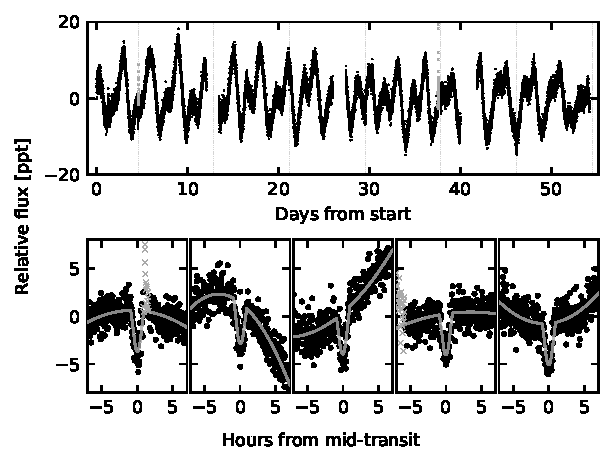
\includegraphics[width=1\textwidth]{f1.pdf}
	\end{center}
	\vspace{-0.7cm}
	\caption{
    {\bf TESS lightcurve of \tn\ (Sectors 10 and 11).}
    {\it Top}: \texttt{PDCSAP} mean-subtracted relative flux at
    2-minute sampling. Spot-induced stellar variability is the
    dominant signal.  Dashed lines show the five transits observed by
    TESS.
    {\it Bottom}: Zoomed windows of individual transits.  Red points
    show manually identified stellar flares.
		\label{fig:rawzoom}
	}
\end{figure*}

%TODO: the scale of this plot is off. (Different font-sizes from
%subplots).
\begin{figure*}[t]
	\begin{center}
		\leavevmode
		\subfloat{
			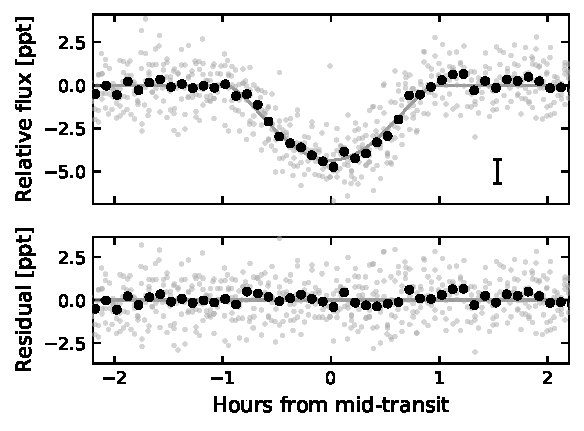
\includegraphics[width=0.7\textwidth]{f2a.pdf}
		}
		
		\vspace{-0.5cm}
		\subfloat{
			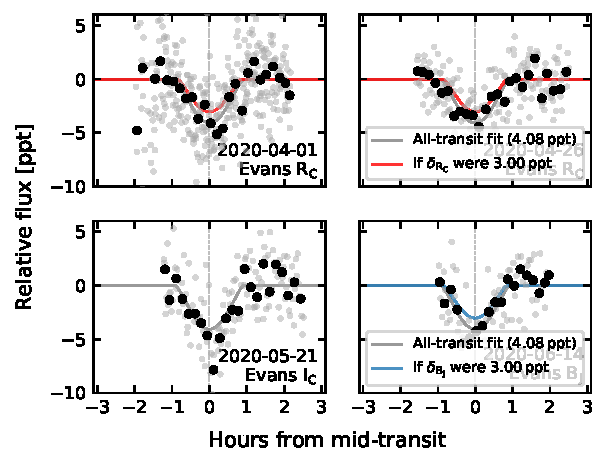
\includegraphics[width=0.7\textwidth]{f2b.pdf}
		}
	\end{center}
	\vspace{-0.7cm}
	\caption{ {\bf Joint TESS and multicolor photometry.}
    {\it Top:} Phase-folded TESS transit. Gray points are 2-minute
    PDCSAP flux measurements, detrended with a 0.3-day robust Huber
    spline (see Section~\ref{subsec:tess}).  Black points are binned
    to 6 minute intervals.  The line shows the transit model
    corresponding to the median transit parameters (Table~2).
    {\it Bottom:} Multicolor photometry from the El Sauce 0.36m.
    The consistent transit depths between TESS-band and the bluer
    Cousins-R and Johnson-B bandpasses rules out select false positive
    scenarios.
		\label{fig:jointphot}
	}
\end{figure*}

\begin{figure}[t!]
	\begin{center}
		\leavevmode
		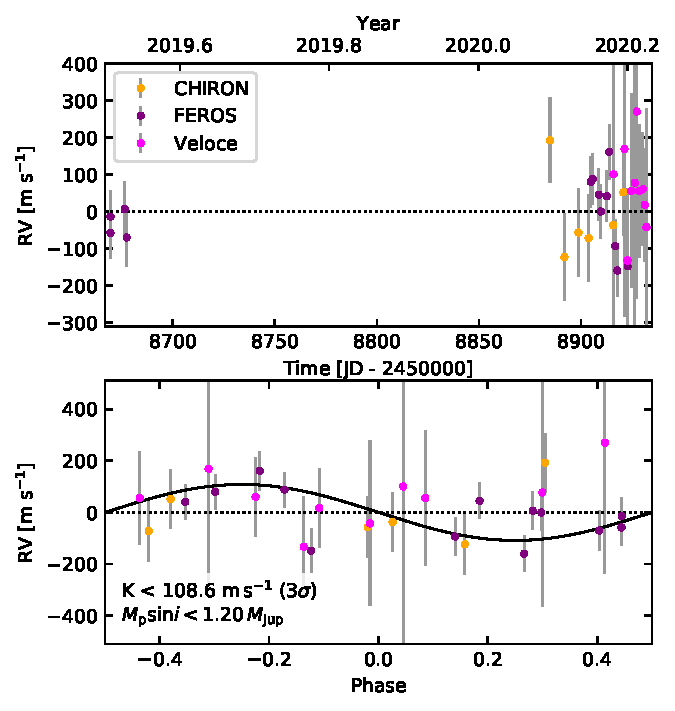
\includegraphics[width=0.47\textwidth]{f3.pdf}
	\end{center}
	\vspace{-0.7cm}
	\caption{
		{\bf Radial velocities.}
		\label{fig:rvs}
	}
\end{figure}

\begin{figure*}[t!]
	\begin{center}
		\leavevmode
		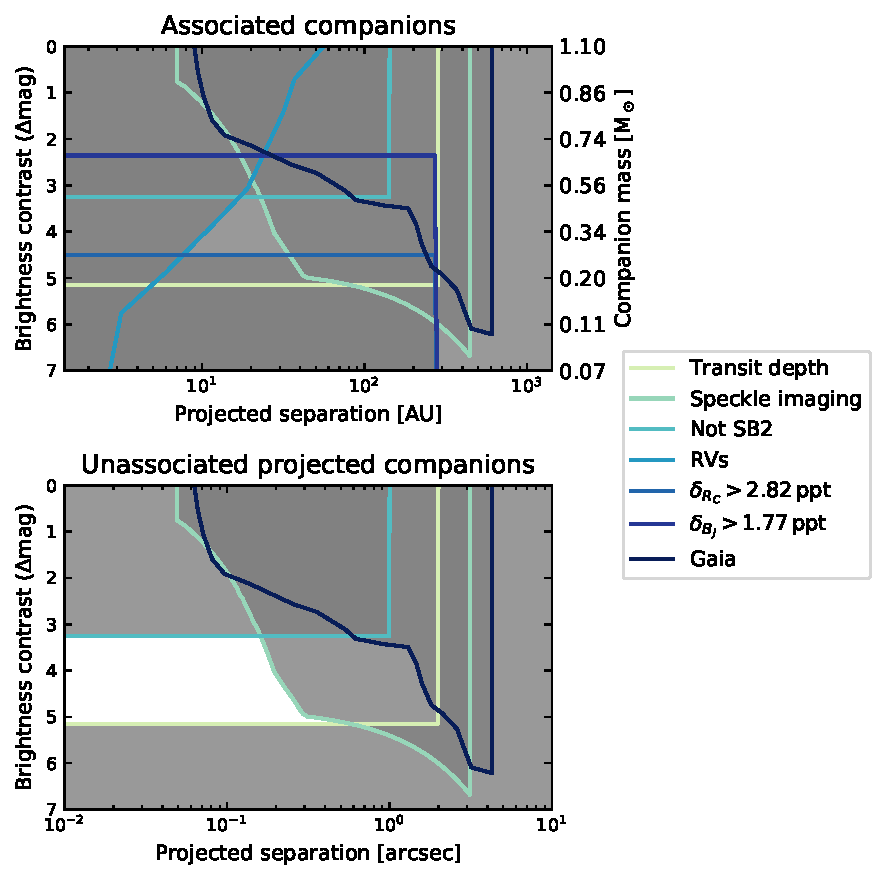
\includegraphics[width=1\textwidth]{f4.pdf}
	\end{center}
	\vspace{-0.7cm}
	\caption{
		{\bf Astrophysical false positive scenarios.}
		{\it Top}: for bound companions,
		{\it Bottom}: for unassociated companions along the same line of
		sight.
		\label{fig:fpscenario}
	}
\end{figure*}

\begin{figure}[t]
	\begin{center}
		\leavevmode
		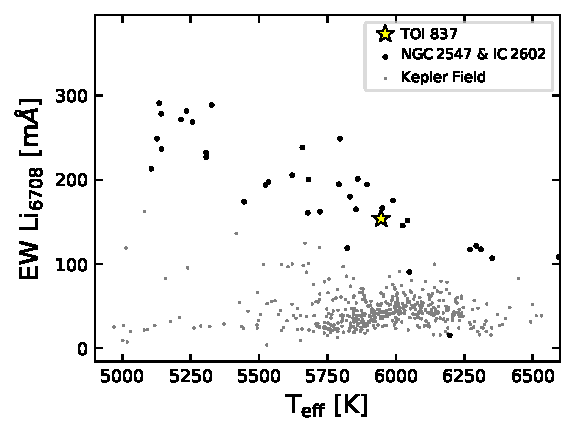
\includegraphics[width=0.45\textwidth]{f5.pdf}
	\end{center}
	\vspace{-0.7cm}
	\caption{ {\bf Scene used for blend analysis.}
		{\it Top:} Mean TESS image of \tn\ over Sector~10, with a
		logarithmic grayscale. The yellow star is the position of \tn.
		Orange circles are neighboring stars with $T<16$, scaled such that
		brighter stars are larger. The \texttt{X} and \texttt{/} hatches
		show the apertures used to measure the background and target star
		flux, respectively. Dashed lines of constant declination and right
		ascension are shown.  {\it Bottom:} Digitized Sky Survey $R$-band
		image of the same field, with a linear grayscale. The circles show
		apertures of radii 1, 1.5, and 2.25 pixels used in our blend
		analysis (Section~\ref{subsec:validation}).  Two stars of interest
		are ``Star A'' and ``Star B'', which were eventually excluded as
		being possible sources of the transits.
		\label{fig:scene}
	}
\end{figure}

\begin{figure}[t]
	\begin{center}
		\leavevmode
		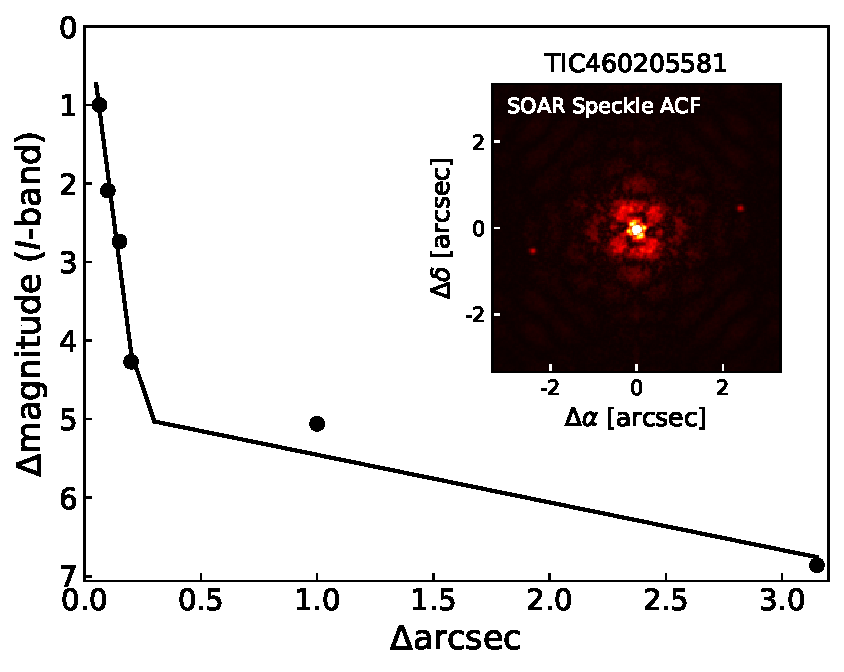
\includegraphics[width=0.45\textwidth]{f6.pdf}
	\end{center}
	\vspace{-0.7cm}
	\caption{ 
		{\bf SOAR HRCam contrast limits derived from point-source
			injection-recovery experiments.} 
		Star A ($\Delta T=4.7$, $\rho=2.3$'' west) is detected in the
		autocorrelation function, in addition to being a resolved Gaia
		source.
		It is co-moving with \tn, and
		its parallax and on-sky position imply that
		it is physically separated from \tn\ by $6.6\pm 0.1\,{\rm pc}$.
		\label{fig:soar}
	}
\end{figure}

\begin{figure}[t!]
	\begin{center}
		\leavevmode
		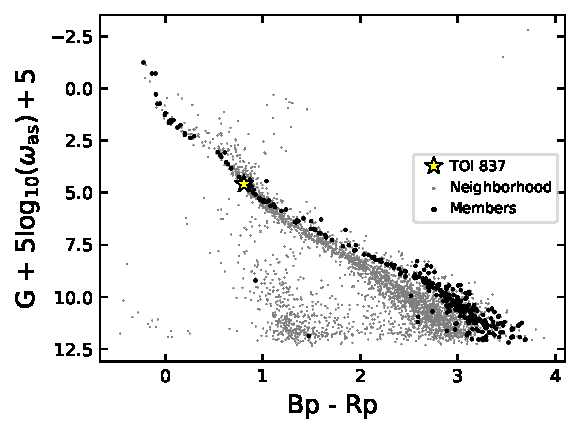
\includegraphics[width=0.45\textwidth]{f7.pdf}
	\end{center}
	\vspace{-0.7cm}
	\caption{ 
  {\bf Hertzsprung-Russell diagram of \tn\ and members of \cn.}
  Members (black circles) were identified by
  \citet{cantatgaudin_gaia_2018}.  Gray circles are non-member stars
  within 5 standard deviations of the mean \cn\ right ascension,
  declination, and parallax.  $G$ denotes Gaia broadband magnitudes,
  $Bp$ Gaia blue, $Rp$ Gaia red, and $\omega_{\rm as}$ the parallax in
  arcseconds. 
  \label{fig:hr}
	}
\end{figure}

\begin{figure*}[t!]
	\begin{center}
		\leavevmode
		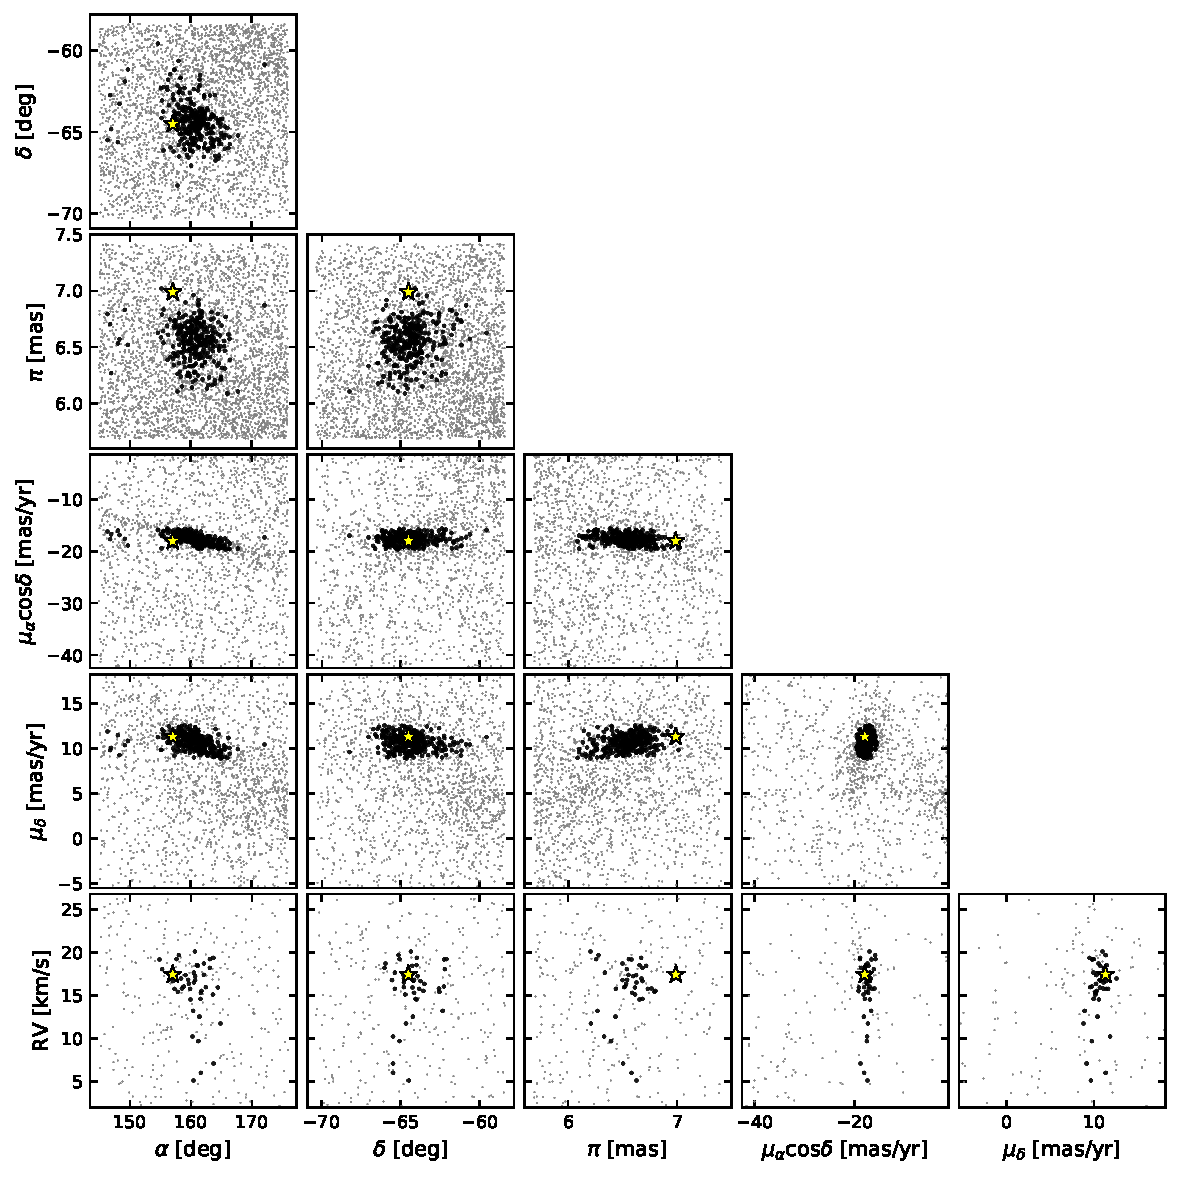
\includegraphics[width=0.9\textwidth]{f8.pdf}
	\end{center}
	\vspace{-0.7cm}
	\caption{ 
  {\bf Positions and kinematics of \tn\ (star), \cn\ members (black
  circles), and stars in the neighborhood (gray circles).} Members
  were identified by \citet{cantatgaudin_gaia_2018}.  $\alpha$ denotes
  right ascension, $\delta$ declination, $\pi$ parallax, $\mu_{\rm
  delta}$ and $\mu_{\rm \alpha}$ proper motion in each equatorial
  direction, and ${\rm RV}$ radial velocity reported by Gaia-DR2.  The
  RVs are for unblended spectra of bright stars ($G\lesssim 12$).  The
  proper motion projection ($\mu_{\delta}$ vs{.} $\mu_{\rm
  \alpha}\cos\delta$) highlights the membership selection function.
  \label{fig:full_kinematics}
	}
\end{figure*}

\begin{figure}[t]
	\begin{center}
		\leavevmode
		\subfloat{
			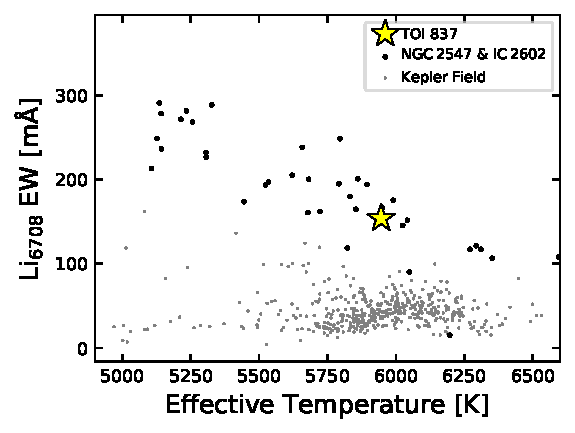
\includegraphics[width=0.45\textwidth]{f9a.pdf}
		}
		
		\vspace{-0.5cm}
		\subfloat{
			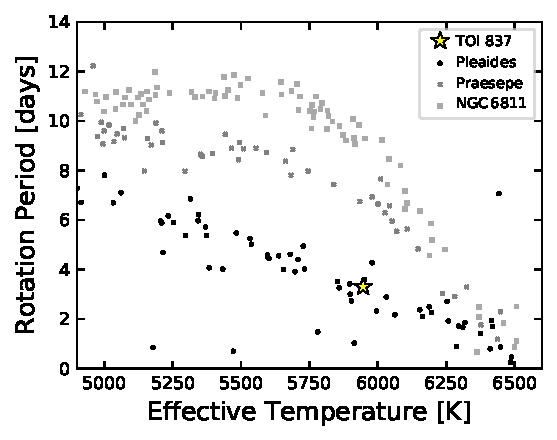
\includegraphics[width=0.45\textwidth]{f9b.pdf}
		}
	\end{center}
	\vspace{-0.7cm}
	\caption{ {\bf Youth diagnostics.}
    {\it Top:} Lithium 6708\AA\ equivalent widths for \tn, field
    stars, and young open clusters.  The field star sample is drawn
    from Kepler planet hosts, and was measured by
    \citet{berger_identifying_2018} using Keck-HIRES.  The young open
    clusters members were surveyed by \citet{randich_gaiaeso_2018}
    using the UVES and GIRAFFE spectrographs at the ESO VLT.
    \citet{randich_gaiaeso_2018} found lithium depletion boundary ages
    for these clusters of $37.7^{+5.7}_{-4.8}\,{\rm Myr}$
    (NGC$\,$2547) and $43.7^{+4.3}_{-3.9}\,{\rm Myr}$ (\cn).  {\it
    Bottom:} Rotation periods for \tn\ and selected open clusters.
    The Pleiades (120$\,$Myr), Praesepe (670$\,$Myr), and NGC$\,$6811
    (1000$\,$Myr) are shown.  Their rotation periods were measured by
    \citet{rebull_rotation_2016a,douglas_poking_2017,douglas_k2_2019},
    and \citet{curtis_temporary_2019}, respectively.
    \label{fig:lithium_rotation}
	}
\end{figure}





\subsection{TESS Photometry}
\label{subsec:tess}

\tn\ (GAIA DR2 5251470948229949568) was observed by the
TESS spacecraft from X to Y in two-minute cadence mode.
The star was designated
TIC\,460205581 in the TESS Input Catalog
\citep{stassun_TIC_2018,stassun_TIC8_2019}.
%FIXME make words more original
The pixel data for an
$11\times11$ array surrounding \tn\ were averaged into 2-minute
stacks by the onboard computer.  Each 2048$\times$2048 image from the
CCD was also averaged into 30-minute stacks, and saved as a ``full
frame image'' (FFI).

%FIXME make words more original
The pixel data for an
The 2-minute stacks for \tn\ were reduced to lightcurves by the
Science Processing Operations Center (SPOC) at NASA
Ames~\citep{jenkins_tess_2016}.  We mainly used the Presearch Data
Conditioning (PDC) lightcurve.  The PDC lightcurve aperture used
pixels chosen to maximize the SNR of the total flux of the target
\citep{smith_finding_2016}.  Non-astrophysical variability
was removed by fitting out trends common to many stars
\citep{smith_kepler_2012,stumpe_multiscale_2014}.

%FIXME make words more original
As an independent check on the 2-minute SPOC lightcurve, we examined
the lightcurve based upon 30-minute image stacks which was produced as
part of the Cluster Difference Imaging Photometric Survey (CDIPS;
\citealt{bouma_cluster_2019}).  Our CDIPS lightcurve of choice used a
circular aperture with radius 1 pixel.


%TODO: describe 0.3-day robust Huber spline

Figure~\ref{fig:rawzoom}.

\subsection{Ground-based Time-Series Photometry}
\label{subsec:groundphot}

  

\subsection{Imaging}

\subsection{Spectroscopy}

\subsubsection{CHIRON}
9 spectra with CTIO1.5/CHIRON, from January 28 through March 14, 2020.
6 were usable.

\subsubsection{FEROS}
N spectra with XXX/FEROS

\subsubsection{Veloce}
M spectra with AAT/Veloce.

\subsection{Astrometry}


\section{Elimination of False Positive Scenarios}
\label{sec:validation}



"""Validation is the process of statistically arguing that a
transit-like signal is due to a planet rather than an astrophysical
false positive. """
(CITE blender, Torres+04,05,10; vespa Morton 12, 15; pastis Diaz+14
Santerne+15; triceratops Giacalone \& Dressing 20).

Many validation analyses are inherently flawed because they do
not deal with the fact that you are conditioned on having observed
many stars, and having found an eclipsing system.

Figure~\ref{fig:fpscenario} provides a visual summary of the possible
astrophysical false positive scenarios.  If the \tn\ signal is not
planetary, it must come from the near-total eclipse of a background
star (a BEB), or else a hierarchical companion of the primary star
(an HEB).  It must also be verified that to the angular resolution
possible, the transit signal originates from \tn, and not a
neighboring star (an NEB).
We proceed by describing each constraint in detail.

\subsection{Limits on Companions from the Transit Depth}

In HEB and BEB scenarios, the flux from \tn\ and the true eclipsing
binary host would blend together, reducing the ``true'' eclipse depth
$\delta_{\rm true}$ to produce the observed depth
$\delta_{\rm obs}$:
\begin{equation}
  \delta_{\rm obs}
  = 
  \delta_{\rm true} \frac{F_{\rm neighbor}}{F_{\rm total}},
\end{equation}
where the total flux and the flux from the neighbor are labelled as
such.  The requirement that the eclipse is produced by stars and that
$\delta_{\rm true} < 0.5$ translates to a bound on the faintest
possible blended companion stars:
\begin{equation}
    \Delta m < - \frac{5}{2} \log_{10} \left( \frac{0.5}{\delta_{\rm obs}} \right).
\end{equation}
For \tn\ ($T=9.93$), this implies that any stellar companion invoked
to explain the transit depth must be brighter than $T=15.07$.

Typically, the shape of the transits enables this argument to be scaled to even
more restrictive depths (e.g., CITE Seager 2003, Vanderburg+2019,
Rizzuto+2020, David+2018 1298Tau).  However, since the transits of
\tn\ are grazing, these arguments do not apply.

\subsection{Limits on Companions from Imaging}

\subsubsection{Gaia Imaging}
Figure~\ref{fig:scene} shows the scene as viewed in the DSS2 plates
and by TESS.  In the upper panels, the pixels used to measure the
background level in the SPOC lightcurve are indicated with
`\texttt{X}' hatching, and the pixels used in the final lightcurve
aperture are shown with `\texttt{/}' hatching.

Stars brighter than $T=16$, as queried from the Gaia DR2 source
catalog, are shown with orange circles.  Given its galactic latitude
of $b=-6^\circ$, it is not surprising that the field of \tn\ is
crowded.  The stars that were of immediate concern for a blend
analysis were as follows.
\begin{itemize}
  \item \tn\ = TIC 460205581 (T=9.9). The target star.
  \item Star A = TIC 847769574 (T=14.6). $2.3$'' west. Proper motions
    and parallax imply it is comoving with \tn, though with a physical
    separation of $6.6\pm 0.1\,{\rm pc}$, it may not be bound.
  \item Star B = TIC 460205587 (T=13.1). $5.4$'' north.  This is a
    giant background star.
\end{itemize}
An additional source, TIC 847769581, is $4.9$'' from the target, but
too faint (T=18.8) to be the source of the observed transit signal.

The Gaia DR2 data for Star A seems poorly behaved.  While
Star A has $G=15.1$, and $Bp=14.9$, no $Rp$ magnitude is reported.
Correspondingly, no RUWE value is available (CITE).  The astrometric
reduced $\chi^2$ ($\chi^2 / (N-5)$, for $N$ the number of good
astrometric observations) seems rather poor, at $8.6$.  We suspect
that the photometric failure to produce an $Rp$ magnitude, as well as
the poor astrometric fit, are likely due to blending with \tn.

At the angular resolution of the TESS data, if either Star A or Star B
were eclipsing binaries, they could be the sources of the transit
signal.  We ruled out both Star A and Star B as hosts of the eclipse
through a detailed analysis of the ground-based seeing-limited
photometry (\S~\ref{subsec:groundphot}).

\subsubsection{Speckle Imaging}

Additional point-sources could be present beyond the angular
resolution of the Gaia source catalog.
To limit this possibility,
we imaged the system using SOAR-HRCam, as described in
\citet{ziegler_soar_2020}.
{\bf Carl: please describe}.
The bandpass was a Johnson-Cousins,
where I is centered at 879 nm and has a width of 289 nm.

Figure~\ref{fig:soar} shows the result.
Star A (TIC 847769574) is detected as expected, and no additional
companions are found.
"""
The points on the plot are measured 5-sigma detectable contrasts. The
lines are linear smoothing fits between two regimes. In general, the
sensitivity of speckle imaging to companions rises sharply from the
diffraction limit to a ``knee'' at a separation of 0.15--0.2
arcseconds, where it then continues to slowly increase out to 1.5$''$,
beyond which the speckle patterns become de-correlated. For this
target, I suspect the measurement at 1$''$ is slightly larger than
expected due to some increase in speckle noise at that radius.
"""

We convert the contrast ratios obtained through the SOAR imaging to
constraints on the masses of putative companions following Montet+2014
(CITE and others!).  We employed the Baraffe+2003 models for
substellar mass objects and the MESA isochrones for stellar mass
objects (Choi et al XXXX).  We assumed that the system age was 35 Myr,
to ensure that companions would be at a plausible state of
contraction.

Due to the specific filters of the SOAR HRcam imager, we further
assumed that all sources had blackbody spectra. While this is clearly
false, we do not readily have access to the planetary and stellar
atmosphere models needed for the correct calculation. However, the
Baraffe+2003 and MESA models do report effective temperatures and
bolometric luminosities.  We opt to use these theoretical quantities,
combined with the measured transmission functions, to calculate the
absolute magnitudes in the HRCam bandpasses (CITE Tokovinin 2018
summary paper with the bandpasses).  

\subsubsection{Patient Imaging}
    Archival SERC-J and AAO-SES plates are available for the \tn\
field\footnote{\url{https://archive.stsci.edu/cgi-bin/dss_form}}.
These plates were acquired in 1982 and 1992, respectively.
For high proper motion stars archival imagery can be used to
detect slowly moving background stars that might be an
astrophysical false-positive source
({\it e.g.}, \citealt{huang_pimen_2018}, CITE VANDERBURG 19).
However \tn\ has only moved $\approx0.7''$ between 1982 and
present, in comparison to the $\approx2.0''$ FWHM of the target on
the plates.
We therefore cannot resolve it with great confidence from
background sources not already resolved through more modern
imaging.

\subsection{Limits on Companions from Radial Velocities}

The combined radial velocities from FEROS, CHIRON, and Veloce 
can be used to place limits on the presence of massive, close-in
bounds companion to \tn.

We derived the relevant limits using \texttt{radvel} \citep{fulton_radvel_2018}.
We assumed circular orbits for the massive companion.
We then fitted the RV data for the semiamplitude, period, time
of conjunction,
instrument offsets, and jitter parameters.
We placed a wide log-uniform prior on the semiamplitude
and period to ensure appropriate sampling of the relevant
spaces.
($\log K \sim \mathcal{U}(1,10^5)$, $\log P \sim \mathcal{U}(0.1, 10^{15})$).

We then converting the resulting posterior in period and semiamplitude
to minimum mass and semi-major axis assuming Kepler's third law.
The resulting $3\sigma$ limits are shown in Figure~\ref{fig:fpscenario}.


\subsection{Limits on Companions from Time-Series Photometry}

\subsubsection{TESS}
We examined the CDIPS FFI lightcurves of the target, which are
available on MAST \citep{bouma_cluster_2019}. Three lightcurves are
available, based on photometric apertures with a radius of 1, 1.5, or
2.5 pixels.  In the raw difference-image light-curves, as well as the
PCA-detrended light-curves, dips of depth $\approx$0.35\% are visible,
and their properties do not significantly vary with aperture size.
Within $\approx20$'', the dips are consistent with originating from
the target star.

\subsubsection{Custom Apertures on Ground-Based Time-Series Photometry}
% See "TOI-837 : a planet!" thread, May 2020

A total eclipse of Star A would produce a 1.4\%
dip. A 30\% eclipse, more plausible for a NEB scenario, would produce
dips of exactly the right depth (0.4\%).

To assess this possibility with the ground-based photometry, we
produced lightcurves centered on \tn\ with
circular apertures of radii ranging from 0.7$''$ to 5.1$''$.
We did not detect any statistically significant variation in the depth
of the transits.

We also created lightcurves with a custom set of $r=2.1''$ apertures
with positions ranging from Star A (2.3$''$ west of \tn) to 2.3$''$
east of \tn.  We did not detect any variation of the transit depth
along this line of lightcurves, as would be expected if Star A were
the eclipse host.  The apertures east of \tn\ are particularly
constraining, as they exclude over 90\% of the flux from Star A.
The eclipse on Star A would therefore need to be excessively deep to
produce the observed eclipse depth.
We take this to indicate that \tn\ is the source of the transit signal
to within $\approx2.0''$.

\newpage
\subsubsection{Color Photometry}

HEB and to a lesser extent BEB scenarios can be limited
by color photometry.
In the absense of color photometry, the most plausible HEB scenarios for TOI
837 involve pairs of eclipsing M dwarfs (Figure~\ref{fig:fpscenario}).
These eclipses are redder than eclipses of the G-dwarf \tn.
Observations that the transit depth does not decrease
going to blue bands therefore limits the plausibility of these scenarios.

\paragraph{Simple Example}
% SEE June 1, 2020 email in "Re: TOI-837.01" thread
As a simple example, assume $M_2=M_3=0.2M_\odot$ in a twin HEB.
Assume PMS evolution, and
use MIST isochrones for a 35 Myr system to convert between stellar properties. 
Take transmission functions (filters only; no instrument or atmosphere
response) from the SVO filter profile service\footnote{\url{http://svo2.cab.inta-csic.es/theory/fps/}}.
Integrate up blackbody functions over each bandpass for each star, and
get estimates of the eclipse depths if there were a total eclipse (of
either of the secondary or tertiary) with this set of parameters.  The
apparent eclipse depths in various Bessel and Cousins bandpasses are:
\begin{align}
%FIXME: check these numbers
  \delta_{\rm U_B} &= 5.03\times10^{-4} \ ({\rm Bessel\ U})\nonumber \\
  \delta_{\rm B_B} &= 1.39\times10^{-3}\ ({\rm Bessel\ B})\nonumber \\
  \delta_{\rm V_B} &= 3.31\times10^{-3}\ ({\rm Bessel\ V})\nonumber \\
  \delta_{\rm R_C} &= 5.59\times10^{-3}\ ({\rm Cousins\ R})\nonumber \\
  \delta_{\rm I_C} &= 9.69\times10^{-3}\ ({\rm Cousins\ I})\nonumber \\
  \delta_{\rm T}   &= 9.18\times10^{-3}\ ({\rm TESS})
\end{align}

Our chief interest is the relative depths, because geometry lets all the
depths be scaled to match the observed TESS depth of $\approx$43 ppt.
(In this case, all depths would be scaled down by a multiplicative factor of
2.1).

The crucial point is that the bluest bands--- U and B---are roughly 10
times shallower than TESS-band, because the M dwarf blackbody function
turns over at 2 times longer wavelengths than the G dwarf blackbody
(Wien's law).

Therefore if TOI 837 were a hierarchical eclipsing M dwarf pair,
Phil's two R-band observations should have shown eclipses a factor of
1.64x shallower than TESS observed (so, 24ppt, instead of the ~40ppt
observed). So, the 40 (+/- 10ish) ppt R-band depths seen in Phil's
transits vs TESS-band argue for a planet, but the level of confidence
could probably be improved with U or B.

\paragraph{Limits on Masses of Bound Companions}

With this intuition in place, we derived the limits on masses of bound
hierarchical eclipsing companions as follows.  We assumed that each
system was composed of the primary (\tn), plus a tertiary companion
eclipsing a secondary companion every 8.3 days.

For secondary masses ranging from 0.07 to 1.10 $M_\odot$, and
mass ratios ($M_3/M_2$) from 0.1 to 1, we then 
calculated the observed maximal eclipse depth of Star 3 in front of
Star 2 in a number of bandpasses.
As before, we interpolated between mass, effective temperature, and radius
assuming the MIST isochrones for a 35$\,$Myr old system,
and also assumed that each source had a blackbody spectrum.

We excluded systems for which the maximal eclipse depth in TESS-band
was less than the observed depth ({\it i.e.}, systems for which the tertiary
was too small).
For the systems with maximal eclipse depths in TESS-band greater than
the observed TESS-band depth, we then calculated the multiplicative
factor required to shrink the depth (from the $b=0$ case) to match the
observed eclipse depth in the TESS-band.
We then scaled the depths in each of the other bandpasses by this
fixed geometric factor.

We then asked: given a fixed secondary mass, are there any tertiary
companions for which the expected $\delta_{\rm R_C}$ is larger than
the observed Rc-band depth?
In cases for which the answer was yes, we could not rule out such
hierarchical eclipsing binary systems.
Conversely, we were able to rule out systems
for which at fixed secondary mass no tertiary mass would
enable eclipses (in ${\rm R_C}$-band) of the necessary depth.

For a lower limit on $\delta_{\rm R_C}$ of 32 parts per thousand,
we found that the transition between systems that would produce
eclipses that no matter what were ``too red'', and systems that would
produce eclipses that could be sufficiently blue happens in \tn\ (for
${\rm R_C}$-band) at 0.54$M_\odot$.
The corresponding limit is shown in Figure~\ref{fig:fpscenario}.

{\bf If we could obtain a similar limit in B-band, it would 
	solidify this result (because it would drive the HEB system to be even bluer).}

\paragraph{Limits on Masses of Projected Companions}

Ignoring the effects of interstellar reddening,
the constraint that $M_2 \gtrsim 0.54 M_\odot$ based on
colors applies to background eclipsing binaries as well.
However, the blue eclipses produced by such systems ({\it e.g.}, a background G2V+K6V binary)
can be kept while making the systems fainter by moving them to greater
distances.
The only way to definitively rule out such scenarios is to 
prove that the loss of light is from the target star,
for instance by detecting the Rossiter-McLaughlin effect
during a transit.

Such scenarios are somewhat contrived in that since 
no secondary eclipse is observed, they require either
eccentric orbits to avoid secondary eclipses, or else a
background twin binary system at double
the orbital period.


\newpage
\subsubsection{Summary}

Possible false-positive scenarios are as follows.

\begin{itemize}
  \item {\it Neighboring blends}.
    Ruled out to within 2 arcseconds by Phil Evans.

  \item {\it Hierarchical blends}.
    Limited by i) FEROS + Veloce RVs, and ii) speckle imaging. 
    Multicolor photometry also limits.

  At present our data do not rule out the presence of bound companion
    stars from $\approx$10--100$\,$AU, with masses in the range of
    $\approx$0.15--0.25$\,$M$_\odot$ (Figure~\ref{fig:fpscenario}).
  Roughly 2-3\% of Sun-like stars in the solar neighborhood with
    binary companions have companions in this region of parameter space
  (assuming the Raghavan+2010 CITE log-normal binary
    separation distribution, and a uniform companion mass function.)

  Companion statistics for hierarchical triples are somewhat less 
    robust, but they have been studied, for instance by CITE
    Tokovinin 2014.
  CITE Tokovinin 2014 found that 7\% of Sun-like stars are
    hierarchical triples with two companions in the compact orbit (the
    ``L$_{12}$'' configuration, rather than the ``L$_{11}$''
    configuration of say, $\alpha$~Centauri).
  A priori then, given a Sun-like primary, the probability that it is in a
    hierarchical triple configuration in which the outer orbit
    satisfies the mass and semi-major axis constraints of
    Figure~\ref{fig:fpscenario} is $\approx 7\% \times 3\% = 0.2\%$. 
  This is independent of the issue that the inner pair would require
    finely tuned orbital parameters (i) to eclipse, and (ii) to
    be so compact.

		

  \item {\it Background blends}.
	An argument on the a priori probability of background blends follows from
	counting statistics. Within 360 arcseconds, there are 298 T<16 stars in TIC8
	(i.e., Gaia DR2). At 2.0 arcseconds, SOAR archives dmag(I) of 6. Inside of 2
	arcseconds, we expect $\pi r^2 $ times (Nstar per sq arcsec) = 9e-3 T<16 stars.
	Any with T$\gtrsim$15 outside of 0.3 arcseconds would have been detected by
	SOAR, which brings down the expected number of possible hidden sources by a
	factor of a few.  Within 0.3 arcseconds, where SOAR gets worse than dmag(I) of
	3, we expect 2e-4 T<16 stars. So (order of magnitude), background blends would
	be a $\sim$0.1\% coincidence.
	%For the background blend to be {\it eclipsing} would require an additional
	%$\sim$2\% coincidence (CITE Kirk+2017 KEBC).
	%Combining the two probabilities yields a prior probability of $\approx$0.002\%.



\end{itemize}



\section{System Modelling}
\label{sec:system}

\subsection{The Cluster}
\label{subsec:cluster}

% NOTE: might want a table of all ages

IC~2602 canonically has an age of $30\pm20\,{\rm Myr}$ (CITE: Van
Leeuwen 2009).
Or logage between 7.533 and 7.563	\citep{bossini_age_2019}.

Or Li age of 40-50Myr (David+19, comparison with other Li stars).

Reported mean metallicity values ${\rm [Fe/H]}$ for the cluster range between
slightly super-solar ($0.04\pm0.01$, \citealt{baratella_gaia-eso_2020}) and
slightly sub-solar ($-0.02 \pm 0.02$, \citealt{netopil_metallicity_2016}).

IC~2602 is supervirial, in the sense that the observed stellar velocity
dispersion is larger than the value expected if it were in virial equilibrium
by about a factor of two \citep{bravi_gaia-eso_2018}.

IC~2602 happens to be near the western edge of the Sco OB2
association, and is relatively close to it in proper motion space
(Damiani+2019).
Damini+2019 also reported evidence for the ongoing evaporation of
\cn, in the form of a diffuse halo of young stars around the central
density cusps.

While \cn\ is older than most known Sco OB2 members,

"""Although IC 2602 does not belong to Sco OB2, it is
spatially and dynamically a close relative, and for this reason
we include it in this work, if even marginally"" (Damiani+2019).
"""We also find that the open cluster IC 2602 has a similar dynamics
to Sco OB2, and its PMS members are currently evaporating and forming
a diffuse (size 10deg) halo around its double-peaked core"""


\subsection{The Star}
\label{subsec:star}
\subsubsection{Cluster Membership}
\label{subsec:member}

\tn\ has been reported as a member of \cn\ by multiple independent 
investigators \citep{Kharchenko_et_al_2013,cantatgaudin_gaia_2018}.
%FIXME FIXME finish these citations
%include: Damiani+2019, Cantat-Gaudin+2020 who explicitly listed it as
%IC2602


The Gaia kinematics are good; gamma velocity is correct; Li (FEROS +
Veloce) is strong; the rotation period and vsini agree with
sub-Pleiades age expected for an IC 2602 member.

\subsubsection{HR Diagram}

Figure~\ref{fig:hr} shows a Hertzsprung-Russell diagram of \tn\ in
reference to the broader \cn\ cluster, as well as its neighborhood.
Cluster members were identified by \citet{cantatgaudin_gaia_2018}
using using Gaia-DR2 positions, proper motions, and parallaxes.  
We included candidate members with formal membership probability
exceeding 10\%.  Save for a few low-mass outliers, most members appear
to be young and coeval.

\tn\ is in its expected position relative to the other members along
the cluster isochrone.  This photometrically limits the presence of
binary companions in the \tn\ system, to a magnitude difference of
perhaps half the brightness of the target star.

Figure~\ref{fig:hr} also suggests that the membership census of \cn\
is incomplete.  We defined the reference ``neighborhood'' as the group
of at most $10^4$ randomly selected non-member stars within 5 standard
deviations of the mean \cn\ right ascension, declination, and
parallax.  We queried Gaia DR2 for these stars using
\texttt{astroquery} \citep{astroquery_2018}.  Many low-mass stars
appear above the main sequence, even though they were not identified
as 5-dimensional kinematic members through the unsupervised
\citet{cantat-gaudin_gaia_2018} membership assignment process.


\subsubsection{Position and Kinematics}

We examine the six-dimensional positions and kinematics in greater
depth in Figure~\ref{fig:full_kinematics}.  The ``neighborhood'' is
defined here identically to as in Figure~\ref{fig:hr}.  The axes
limits for the right ascension, declination, and parallax dimensions
are as in the Gaia archive query.  The axes limits for the proper
motion and radial velocity dimensions are set at the 25$^{\rm th}$ and
75$^{\rm th}$ percentiles, in order to give a sense of the
population's distribution, while excluding outlying points.  The
radial velocities suffer the greatest incompleteness due to the
current $G\approx12$ magnitude limit of the Gaia-DR2 data processing.

Figure~\ref{fig:full_kinematics} provides strong evidence {\it (i)} for the
existence of the \cn\ open cluster and {\it (ii)} for the membership
of \tn\ within \cn.
The only dimension that could perhaps lead to some worry is the
parallax, as \tn\ is one of the closest \cn\ members reported by
\citet{cantatgaudin_gaia_2018}.
Fortunately, there are independent means of verifying stellar youth.


\subsubsection{Rotation}

TESS photometric rotation period = 3.5days ish.
vsini = 17.48 $\pm$ 0.15 (CHIRON).
The two agree.

For comparison, gyrochrones would ``predict'' X.XX.

This implies sub-Pleiades age expected for an IC 2602 member.

Figure~\ref{fig:lithium_rotation} compares the stellar rotation period of \tn\ to
periods that have been measured in a number of well-studied open clusters.
\tn\ seems to be gyrochronologically coeval with the Pleiades sequence.

We note that this is still in the ``sub 500 Myr'' range, when classical
Skumanich spin-down is not expected to be happening (why is this the number?).

This agrees with recent empirical results from Rebull et al 2020 and perhaps also 2018(?):
they observed the Taurus foreground (age 30 Myr) and saw that it was 
roughly consistent with the Pleaides.
Upper Sco had a consistent mean, but a much larger scatter.

%NOTE: begs the question... is there a large population of ~30-50 Myr old
% stars for which we could measure the rotation periods, and clarify if the scatter of Upper Sco chills out?


\subsubsection{Lithium}

Rafael's co-added FEROS spectra gave a Li doublet equivalent width of
154 milliangstrom.

Lithium depletion for a star of TOI-837's spectral type happens
over timescales >100 Myr (Soderblom+2013). This is because the
convective envelopes are very shallow, so they don't cycle material
down to the >3e6 K core until much later.

Nonetheless, comparison of early-G field stars to e.g., 600 Myr old
Hyads has shown that the depletion does happen over gigayear timescales
(Berger+2018, fig 7).

Figure~\ref{fig:lithium_rotation} compares our measured \tn\ Li EW 
to stars in the field, and to young open cluster members.
The field star measurements were collected by
\citet{berger_identifying_2018}.
We have shown the points with lithium detections at ${\rm SNR}>3$.
TOI-837 is consistent with being younger than almost all CKS
planet-hosting field stars.

The young open cluster members were selected for the presence of
lithium, as described by \citet{randich_gaiaeso_2018}.
The TOI-837 Li EW measured here (150 milliangstrom) is consistent
with what's seen for stars of similar colors in <100 Myr old moving
groups.
(Elliott+2016, Fig 11 -- attached).  This is sensible, because
IC 2602 is supposed to be 50 Myr old.



\subsubsection{Literature Membership}
The membership of \tn\ in \cn\ was noted by \citet{oh_comoving_2017},
in what they dubbed ``Group 5''.
Analyzing the clusters of \citet{oh_comoving_2017},
\citet{bochanski_fundamental_2018} fitted the Gaia, 2MASS, and
WISE photometry with MIST isochrones, and reported stellar masses,
radii, metallicities, ages, distances, and extinction for 9754 stars,
including \tn.
%Bochanski reported:
%logAge 9.38 +0.42 -0.26
%dist 138.3 +7.0 -7.2
%A_v = 0.27 +0.18 - 0.18
%


\tn\ was also listed as a member of ``Theia 92'' by
\citet{kounkel_untangling_2019}.
These authors identified 999 candidate cluster members, and
reported a cluster isochrone age $\log t = 7.55$ with uncertainty
$\approx 0.15\,{\rm dex}$.
They reported an average extinction of Av=0.243 mag.


\subsubsection{Stellar Parameters}

% TODO: decide whether to include

% \begin{figure}[t!]
% 	\begin{center}
% 		\leavevmode
% 		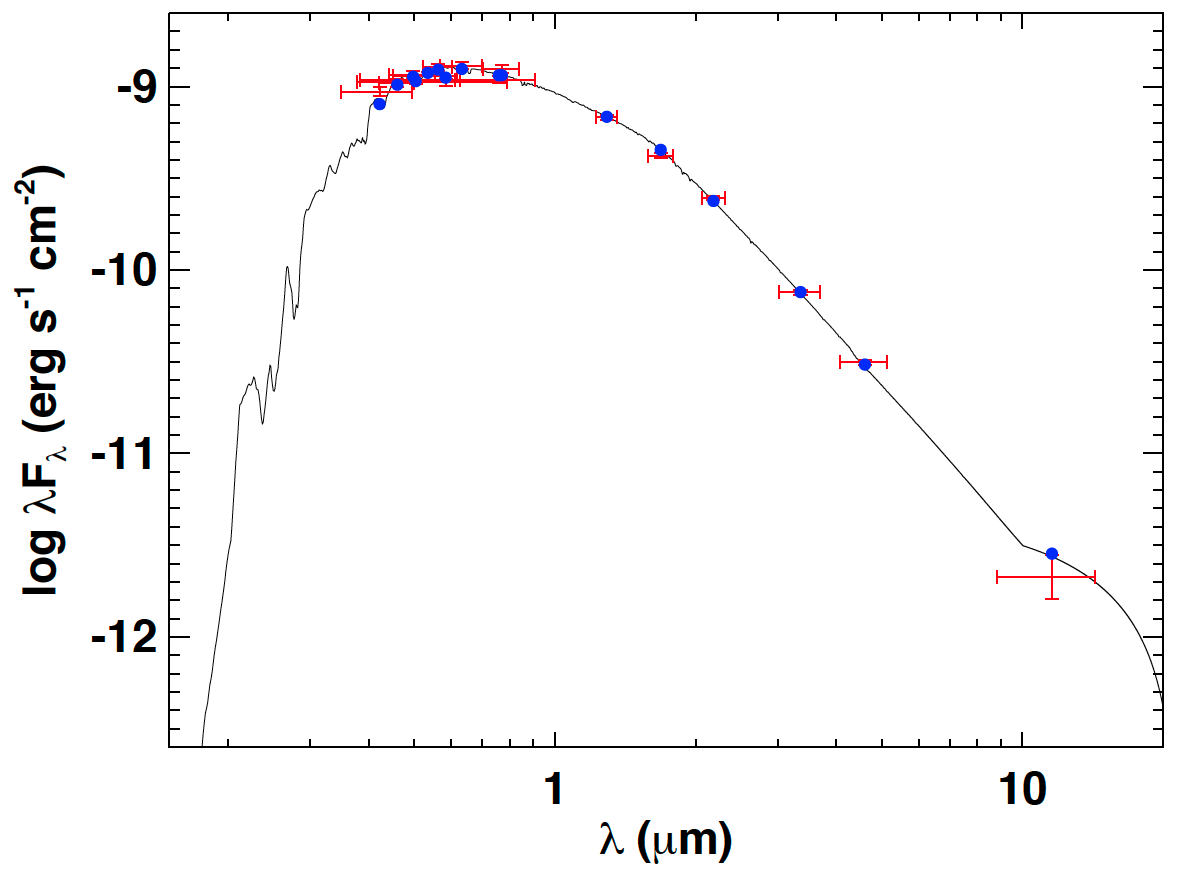
\includegraphics[width=0.48\textwidth]{f6.png}
% 	\end{center}
% 	\vspace{-0.7cm}
% 	\caption{
%     {\bf Spectral energy distribution of \tn\ from archival
%     photometry.}
%     {\bf Keivan: please describe, and if possible, send me the data
%     (photometry + the atmosphere model) used to generate the plot so I
%     can regenerate it in a consistent style with the rest of the paper}
%     \label{fig:sed}
% 	}
% \end{figure}

\subsubsection{Physical}
 (Lstar, Rstar, Teff, Age and Mstar)

From CHIRON spectra, my current best guess spectroscopic parameters
 are as follows.
 Teff = 5946 +/- 39
 logg = 4.48 +/- 0.03
 feh = -0.065 +/- 0.035
 vsini = 17.48 +/- 0.15

Figure~\ref{fig:sed}.
The SED fit, looking really good with rchi2 = 1.6: 

The fit parameters are: 
Av = 0.20 +/- 0.03
Fbol = 1.967 +/- 0.046 e-9 erg/s/cm2 
Rstar = 1.049 +/- 0.019 Rsun 

From the spectroscopic logg and the above Rstar, we get an independent
mass estimate of 
Mstar = 1.21 +/- 0.10 Msun 
At face value, the mass seems a bit high for the radius, but I'm
guessing that just means the spectroscopic logg is a bit too high. 


\paragraph{Astrometric information}
The RUWE (CITE, CITE) for \tn\ is 1.02, indicative that there are no
obviously present astometric companions.


\subsubsection{Rotation}
Stellar vsini
Stellar rotation

\subsubsection{RVs}
I don't strongly expect the Veloce RVs or the FEROS ones to lead to a
mass measurement. The reason is that with vsini=17km/s, and 2\%
rotation amplitude signal, we expect an RV RMS of 300m/s at the
Prot=3.5 day rotation period (vsini*rotation amplitude). This is
probably larger than the expected planet signal (100m/s, 8 days).




\subsection{The Planet}
\label{subsec:planet}

\subsubsection{Transit Fitting}
Simultaneous dip plus rotation period (GP) fit. Use celerite plus PyMC3/exoplanet.
Mention FPP?


\subsubsection{Additional Transits}

None of the extra dips in the PDCSAP light-curve (e.g., ``up-down''
spikes at BTJD 1572 and 1601) seem likely to be planetary
We checked that i) they were not present in the SAPFLUX light-curves,
and ii) that they were not present in the CDIPS light-curves (either
raw, or PCA-detrended).

To make this quantitative, we did injection-recovery.



\section{Discussion}
\label{sec:discussion}

Rossiter measurements will confirm.

After, a mass measurement should be worthwhile.

We'll get more TESS data in January(?).




%%%%%%%%%%%%%%%%%%%%%%%%%%%%%%%%%%%%%%%%%%%%%%%%%%%%%%%%%%%%%%%%%%%%%%%%%%%%%%%

\acknowledgements
%
%This paper includes data collected by the TESS mission, which are
%publicly available from the Mikulski Archive for Space Telescopes
%(MAST).
%
%Funding for the TESS mission is provided by NASA's Science Mission
%directorate.
%
The authors thank...
%
We also thank the Heising-Simons Foundation for
their generous support of this work.
%
The Digitized Sky Survey was produced at the Space Telescope Science
Institute under U.S. Government grant NAG W-2166.
Figure~\ref{fig:scene} is based on photographic data obtained using
the Oschin Schmidt Telescope on Palomar Mountain.
%
This research made use of the Exoplanet Follow-up Observation
Program website, which is operated by the California Institute of
Technology, under contract with the National Aeronautics and Space
Administration under the Exoplanet Exploration Program.
%
This research has made use of the SVO Filter Profile Service
(\url{http://svo2.cab.inta-csic.es/theory/fps/}) supported from the Spanish
MINECO through grant AYA2017-84089
%
% %
% Based on observations obtained at the Gemini Observatory, which is
% operated by the Association of Universities for Research in Astronomy,
% Inc., under a cooperative agreement with the NSF on behalf of the
% Gemini partnership: the National Science Foundation (United States),
% National Research Council (Canada), CONICYT (Chile), Ministerio de
% Ciencia, Tecnolog\'{i}a e Innovaci\'{o}n Productiva (Argentina),
% Minist\'{e}rio da Ci\^{e}ncia, Tecnologia e Inova\c{c}\~{a}o (Brazil),
% and Korea Astronomy and Space Science Institute (Republic of Korea).
% %
% Observations in the paper made use of the High-Resolution Imaging
% instrument Zorro at Gemini-South. Zorro was funded by the NASA
% Exoplanet Exploration Program and built at the NASA Ames Research
% Center by Steve B. Howell, Nic Scott, Elliott P. Horch, and Emmett
% Quigley.
% %
% This research has made use of the VizieR catalogue access tool, CDS,
% Strasbourg, France. The original description of the VizieR service was
% published in A\&AS 143, 23.
% %
% This work has made use of data from the European Space Agency (ESA)
% mission {\it Gaia} (\url{https://www.cosmos.esa.int/gaia}), processed
% by the {\it Gaia} Data Processing and Analysis Consortium (DPAC,
% \url{https://www.cosmos.esa.int/web/gaia/dpac/consortium}). Funding
% for the DPAC has been provided by national institutions, in particular
% the institutions participating in the {\it Gaia} Multilateral
% Agreement.
%
% (Some of) The data presented herein were obtained at the W. M. Keck
% Observatory, which is operated as a scientific partnership among the
% California Institute of Technology, the University of California and
% the National Aeronautics and Space Administration. The Observatory was
% made possible by the generous financial support of the W. M. Keck
% Foundation.
% The authors wish to recognize and acknowledge the very significant
% cultural role and reverence that the summit of Maunakea has always had
% within the indigenous Hawaiian community.  We are most fortunate to
% have the opportunity to conduct observations from this mountain.
%
% \newline
%

\software{
  \texttt{astrobase} \citep{bhatti_astrobase_2018},
  %\texttt{astroplan} \citep{astroplan2018},
  \texttt{astropy} \citep{astropy_2018},
  \texttt{astroquery} \citep{astroquery_2018},
  %\texttt{BATMAN} \citep{kreidberg_batman_2015},
  \texttt{cdips-pipeline} \citep{bhatti_cdips-pipeline_2019}
  \texttt{corner} \citep{corner_2016},
  %\texttt{emcee} \citep{foreman-mackey_emcee_2013},
  \texttt{exoplanet} \citep{exoplanet:agol19}
  \texttt{exoplanet} \citep{exoplanet:exoplanet}, and its
  dependencies \citep{exoplanet:agol19, exoplanet:kipping13, exoplanet:luger18,
  	exoplanet:theano}.
  \texttt{IPython} \citep{perez_2007},
	\texttt{lightkurve} \citep{lightkurve_2018},
  \texttt{matplotlib} \citep{hunter_matplotlib_2007}, 
  \texttt{MESA} \citep{paxton_modules_2011,paxton_modules_2013,paxton_modules_2015}
  \texttt{numpy} \citep{walt_numpy_2011}, 
  \texttt{pandas} \citep{mckinney-proc-scipy-2010},
  \texttt{pyGAM} \citep{serven_pygam_2018_1476122},
  \texttt{PyMC3} \citep{salvatier_2016_PyMC3},
  %\texttt{radvel} \citep{fulton_radvel_2018},
  %\texttt{scikit-learn} \citep{scikit-learn},
  \texttt{scipy} \citep{jones_scipy_2001}.
  \texttt{tesscut} \citep{brasseur_astrocut_2019},
  \texttt{webplotdigitzer} \citep{rohatgi_2019},
  \texttt{wotan} \citep{hippke_wotan_2019}.
}


\facilities{
 	{\it Astrometry}:
 	Gaia \citep{gaia_collaboration_gaia_2016,gaia_collaboration_gaia_2018}.
 	{\it Imaging}:
  Second Generation Digitized Sky Survey,
 	Keck:II~(NIRC2; \url{www2.keck.hawaii.edu/inst/nirc2}).
 	%Gemini:South~(Zorro; \citealt{scott_nessi_2018}.
 	{\it Spectroscopy}:
 	Keck:I~(HIRES; \citealt{vogt_hires_1994}).
 	{\bf VLT (number), UVES and GIRAFFE} (CITE: Pasquini et al 2002)
% 	Euler1.2m~(CORALIE),
% 	ESO:3.6m~(HARPS; \citealt{mayor_setting_2003}).
 	{\it Photometry}:
% 	CTIO:1.0m (Y4KCam),
% 	Danish 1.54m Telescope,
% 	El Sauce:0.356m,
% 	Elizabeth 1.0m at SAAO,
% 	Euler1.2m (EulerCam),
% 	Magellan:Baade (MagIC),
% 	Max Planck:2.2m	(GROND; \citealt{greiner_grond7-channel_2008})
% 	NTT,
% 	SOAR (SOI),
 	TESS \citep{ricker_transiting_2015}.
% 	TRAPPIST \citep{jehin_trappist_2011},
% 	VLT:Antu (FORS2).
}

%
% The following are entries from Table 1 that are not otherwise cited
% in the text
%
% \nocite{wilson_wasp-4b_2008}
% \nocite{gillon_improved_2009}
% \nocite{winn_transit_2009}
% \nocite{hoyer_tramos_2013}
% \nocite{dragomir_terms_2011}
% \nocite{sanchis-ojeda_starspots_2011}
% \nocite{nikolov_wasp-4b_2012}
% \nocite{ranjan_atmospheric_2014}
% \nocite{huitson_gemini_2017}

% \input{WASP-4b_transit_time_table.tex}
% \input{WASP-4b_rv_table.tex}
% \input{model_fit_table.tex}
% \input{rv_model_posterior_table.tex}
% \input{pdot_table.tex}

\clearpage
\startlongtable
\begin{deluxetable*}{lrrrrrrrr}
%
%\tabletypesize{\scriptsize}
%
\tablenum{1}
%
\tablecaption{Model Comparison.}
\label{tab:modelcompare}
%
\tablehead{
\colhead{Description} &
\colhead{$N_{\rm s}$} &
\colhead{$N_{\rm \ell}$} &
\colhead{$N_{\rm data}$} &
\colhead{$N_{\rm param}$} &
\colhead{$\chi^2$} &
\colhead{$\chi_{\rm red}^2$} &
\colhead{BIC} &
\colhead{$\Delta$BIC}
}
% pasted from
% /Users/luke/Dropbox/proj/billy/results/PTFO_8-8695_results/20200428_v0/bic_table_data.tex
% 
% Burnham and Anderson 2004.
% "Models having i ≤ 2 have substantial support (evidence), those in which 4 ≤
% i ≤ 7 have considerably less support, and models having i > 10 have
% essentially no support"
\startdata
Favored    & 2 &  2 &   2585 &      17 &  3230.2 &     1.258 &  3363.7 &     0.0 \\
\hline
Weakly favored &  3 &  3 &   2585 &      21 &  3203.4 &     1.249 &  3368.4 &     4.7 \\
---               & 3 &  2 &   2585 &      19 &  3222.9 &     1.256 &  3372.2 &     8.4 \\
\hline
Disfavored      & 2 &  3 &   2585 &      19 &  3244.9 &     1.265 &  3394.2 &    30.4 \\
---              & 2 &  1 &   2585 &      15 &  3410.6 &     1.327 &  3528.5 &   164.7 \\
---             &  3 &  1 &   2585 &      17 &  3396.4 &     1.323 &  3530.0 &   166.3 \\
---             & 1 &  2 &   2585 &      15 &  4158.6 &     1.618 &  4276.4 &   912.7 \\
---             & 1 &  3 &   2585 &      17 &  4147.4 &     1.615 &  4281.0 &   917.2 \\
---            &  1 &  1 &   2585 &      13 &  4313.5 &     1.677 &  4415.6 &  1051.9 \\
\enddata
%
\tablecomments{
	$N_{\rm s}$ and $N_{\rm \ell}$ are the number of harmonics at the short and long periods, respectively.
	$N_{\rm data}$ is the number of fitted flux measurements.
	$N_{\rm param}$ is the number of free parameters in the model.
	The Bayesian information criterion (BIC) and the difference from the maximum $\Delta {\rm BIC}$ are also listed.
}
\vspace{-1cm}
\end{deluxetable*}

% Table of best fit parameters
%\startlongtable
\begin{deluxetable*}{lllrrrrr}
%
  \tablecaption{ Priors and posteriors for the model fitted to the
  TESS data.}
\label{tab:posterior}
%
%\tabletypesize{\scriptsize}
%
%\tablenum{2}
%
\tablehead{
  \colhead{Param.} & 
  \colhead{Unit} &
  \colhead{Prior} & 
  \colhead{Median} & 
  \colhead{Mean} & 
  \colhead{Std{.} Dev.} &
  \colhead{3\%} &
  \colhead{97\%}
}

% /Users/luke/Dropbox/proj/timmy/results/TOI_837_tessindivtransit_phot_results/20200711/posterior_table_clean_tessindivtransit.tex
\startdata
$P$ & d & $\mathcal{N}(8.3249; 0.1000)$ & 8.3247158 & 8.3247141 & 0.0003210 & 8.3240946 & 8.3253007 \\
$t_0^{(1)}$ & d & $\mathcal{N}(1574.273800; 0.1000)$ & 1574.2730012 & 1574.2730125 & 0.0010420 & 1574.2710233 & 1574.2749496 \\
$\log R_{\rm p}/R_\star$ & -- & $\mathcal{U}(-4.605; 0.000)$ & -2.51877 & -2.50605 & 0.09466 & -2.66494 & -2.32807 \\
$b$ & -- & $\mathcal{U}(0; 1+R_{\mathrm{p}}/R_\star)$ & 0.9521 & 0.9536 & 0.0125 & 0.9318 & 0.9768 \\
$u_1$ & -- & $\mathcal{U}(0.175; 0.475)$$^{(2)}$ & 0.335 & 0.332 & 0.086 & 0.196 & 0.475 \\
$u_2$ & -- & $\mathcal{U}(0.085; 0.385)$$^{(2)}$ & 0.243 & 0.240 & 0.086 & 0.105 & 0.384 \\
$R_\star$ & $R_\odot$ & $\mathcal{T}(1.022; 0.015)$ & 1.022 & 1.022 & 0.015 & 0.994 & 1.050 \\
$\log g$ & cgs & $\mathcal{N}(4.467; 0.010)$ & 4.467 & 4.467 & 0.010 & 4.448 & 4.486 \\
$a_{00;\mathrm{TESS}}$ & -- & $\mathcal{N}(1.00; 0.01)$ & 0.9985 & 0.9985 & 0.0001 & 0.9983 & 0.9986 \\
$a_{01;\mathrm{TESS}}$ & d$^{-1}$ & $\mathcal{U}(-0.05; 0.05)$ & -0.0004 & -0.0004 & 0.0003 & -0.0011 & 0.0002 \\
$a_{02;\mathrm{TESS}}$ & d$^{-2}$ & $\mathcal{U}(-0.05; 0.05)$ & -0.0168 & -0.0168 & 0.0023 & -0.0211 & -0.0124 \\
$a_{10;\mathrm{TESS}}$ & -- & $\mathcal{N}(1.00; 0.01)$ & 1.0089 & 1.0089 & 0.0001 & 1.0088 & 1.0091 \\
$a_{11;\mathrm{TESS}}$ & d$^{-1}$ & $\mathcal{U}(-0.05; 0.05)$ & -0.0138 & -0.0138 & 0.0003 & -0.0144 & -0.0132 \\
$a_{12;\mathrm{TESS}}$ & d$^{-2}$ & $\mathcal{U}(-0.05; 0.05)$ & -0.0536 & -0.0536 & 0.0022 & -0.0577 & -0.0494 \\
$a_{20;\mathrm{TESS}}$ & -- & $\mathcal{N}(1.00; 0.01)$ & 0.9991 & 0.9991 & 0.0001 & 0.9989 & 0.9993 \\
$a_{21;\mathrm{TESS}}$ & d$^{-1}$ & $\mathcal{U}(-0.05; 0.05)$ & 0.0156 & 0.0156 & 0.0004 & 0.0150 & 0.0163 \\
$a_{22;\mathrm{TESS}}$ & d$^{-2}$ & $\mathcal{U}(-0.05; 0.05)$ & 0.0246 & 0.0246 & 0.0024 & 0.02 & 0.0289 \\
$a_{30;\mathrm{TESS}}$ & -- & $\mathcal{N}(1.00; 0.01)$ & 1.0012 & 1.0012 & 0.0001 & 1.0010 & 1.0014 \\
$a_{31;\mathrm{TESS}}$ & d$^{-1}$ & $\mathcal{U}(-0.05; 0.05)$ & 0.0021 & 0.0021 & 0.0004 & 0.0014 & 0.0029 \\
$a_{32;\mathrm{TESS}}$ & d$^{-2}$ & $\mathcal{U}(-0.05; 0.05)$ & -0.0079 & -0.0079 & 0.0029 & -0.0133 & -0.0025 \\
$a_{40;\mathrm{TESS}}$ & -- & $\mathcal{N}(1.00; 0.01)$ & 0.9906 & 0.9906 & 0.0001 & 0.9904 & 0.9907 \\
$a_{41;\mathrm{TESS}}$ & d$^{-1}$ & $\mathcal{U}(-0.05; 0.05)$ & 0.0015 & 0.0015 & 0.0003 & 0.0009 & 0.0022 \\
$a_{42;\mathrm{TESS}}$ & d$^{-2}$ & $\mathcal{U}(-0.05; 0.05)$ & 0.0327 & 0.0327 & 0.0023 & 0.0283 & 0.0370 \\
$R_{\rm p}/R_\star$ & -- & -- & 0.08 & 0.08 & 0.01 & 0.07 & 0.10 \\
$\rho_\star$ & g$\ $cm$^{-3}$ & -- & 1.47 & 1.47 & 0.04 & 1.40 & 1.55 \\
$R_{\rm p}$ & $R_{\mathrm{Jup}}$ & -- & 0.80 & 0.82 & 0.08 & 0.68 & 0.97 \\
$a/R_\star$ & -- & -- & 17.54 & 17.54 & 0.16 & 17.24 & 17.84 \\
$\cos i$ & -- & -- & 0.05 & 0.05 & 0. & 0.05 & 0.06 \\
$T_{14}$ & hr & -- & 1.85 & 1.86 & 0.04 & 1.78 & 1.93 \\
$T_{13}$ & hr & -- & 0.20 & 0.21 & 0.10 & 0.01 & NaN$^{(3)}$ \\
\enddata
%
\tablecomments{
(1) For the most precise ephemeris based on the combination of TESS and
ground-based data, please see Equation~\ref{eq:ephem}; the period and epoch are noted
in this table only for self-consistency.
%
% (2) Uninformative quadratic limb-darkening prior from \citet{exoplanet:kipping13}, implemented by \citet{exoplanet:exoplanet}.
% The precision achieved in the ground-based data did not appear to
% necessitate using bandpass-dependent limb-darkening coefficients.
% For comparison, the \citet{claret_limb_2017} parameters for
% the appropriate $T_{\rm eff}$ and $\log g$ in TESS-band would have been 
% $(u_1, u_2) = (0.3249, 0.235)$.
%
(2) Assuming an informative quadratic limb-darkening prior with
values about those given for the appropriate $T_{\rm eff}$ and
$\log g$ in TESS-band from \citet{claret_limb_2017}. The precision
achieved in the ground-based data did not appear to necessitate using
bandpass-dependent limb-darkening coefficients.
(3) The second and third contact points do not exist for a grazing transit.
{\it Notation}:
$a_{ij;\mathrm{Instr}}$ denotes the $i^{\rm th}$ transit of a
particular instrument, and the $j^{\rm th}$ polynomial detrending
order.
$\mathcal{U}$ denotes a uniform distribution,
$\mathcal{N}$ a normal distribution, and
$\mathcal{T}$ a truncated normal bounded between zero and an upper limit much larger than the mean.
}
\vspace{-0.3cm}
\end{deluxetable*}

\clearpage

\bibliographystyle{yahapj}                            
\bibliography{bibliography} 

% \appendix
% \section{Gaia query}
% bounding by 5 stdevns
% Launched query: '
%         select top 10000
%             g.source_id, g.phot_bp_mean_mag, g.phot_rp_mean_mag,
%             g.phot_g_mean_mag, g.parallax, g.ra, g.dec, g.pmra, g.pmdec,
%             g.radial_velocity, g.radial_velocity_error
%         from gaiadr2.gaia_source as g
%         where
%             g.parallax > 5.69
%         and
%             g.parallax < 7.41
%         and
%             g.dec < -58.41
%         and
%             g.dec > -70.33
%         and
%             g.ra > 145.01
%         and
%             g.ra < 175.85
%         and
%             g.phot_g_mean_mag < 18
%         order by
%             random_index

\listofchanges

\end{document}
